% Created 2015-06-20 Sáb 23:01
\documentclass[11pt]{article}
\usepackage[utf8]{inputenc}
\usepackage[T1]{fontenc}
\usepackage{fixltx2e}
\usepackage{graphicx}
\usepackage{longtable}
\usepackage{float}
\usepackage{wrapfig}
\usepackage{rotating}
\usepackage[normalem]{ulem}
\usepackage{amsmath}
\usepackage{textcomp}
\usepackage{marvosym}
\usepackage{wasysym}
\usepackage{amssymb}
\usepackage{hyperref}
\tolerance=1000
\usepackage{minted}
\usemintedstyle{perldoc}
\usepackage{tikz}
\usetikzlibrary{decorations.markings}
\tikzstyle{vertex}=[circle, draw, inner sep=0pt, minimum size=7pt]
\newcommand{\vertex}{\node[vertex]}
\newcommand{\tu}{\textunderscore}
\author{Alice Duarte Scarpa, Bruno Lucian Costa}
\date{2015-06-23}
\title{Exercício 6.30 (Papadimitriou)}
\hypersetup{
  pdfkeywords={},
  pdfsubject={},
  pdfcreator={Emacs 24.4.1 (Org mode 8.2.10)}}
\begin{document}

\maketitle

\section{Enunciado}
\label{sec-1}

\textit{Reconstruindo árvores filogenéticas pelo método da máxima parcimônia}

Uma árvore filogenética é uma árvore em que as folhas são espécies
diferentes, cuja raiz é o ancestral comum de tais espécies e cujos
galhos representam eventos de especiação.

Queremos achar:

\begin{itemize}
\item Uma árvore (binária) evolucionária com as espécies dadas
\item Para cada nó interno uma string de comprimento $k$ com a
sequência genética daquele ancestral.
\end{itemize}


Dada uma árvore acompanhada de uma string $s(u) \in \{A, C, G, T\}^k$ para
cada nó $u \in V(T)$, podemos atribuir uma nota usando o método da
máxima parcimônia, que diz que menos mutações são mais prováveis:
\[ \mathrm{nota}(T) = \sum_{(u,v) \in E(T)} (\text{número de posições em que }s(u)\text{ e }s(v)\text{ diferem}). \]

Achar a árvore com nota mais baixa é um problema difícil. Aqui vamos
considerar um problema menor: Dada a estrutura da árvore, achar as
sequências genéticas $s(u)$ para os nós internos que dêem a nota mais
baixa.

Um exemplo com $k = 4$ e $n = 5$:

\href{http://github.com/adusca/FGV-EDA/6_30/tree.png}{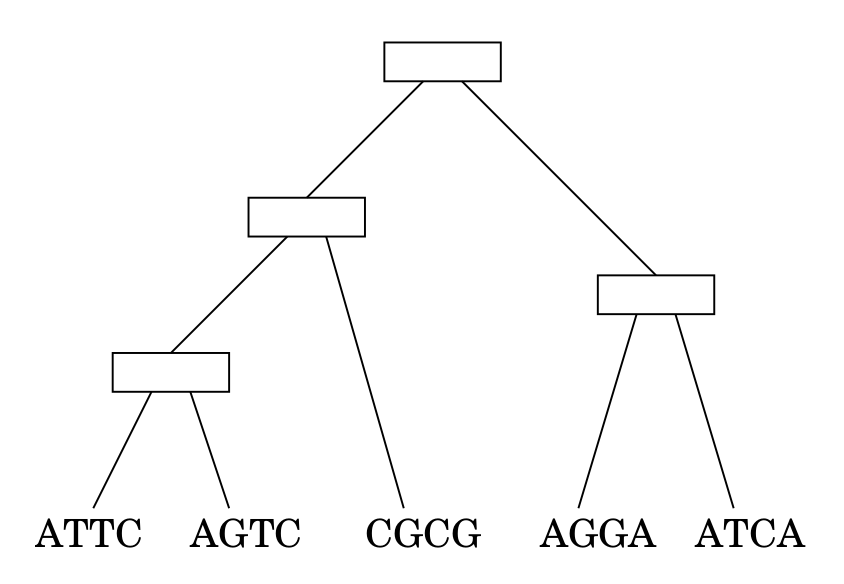
\includegraphics[width=.9\linewidth]{tree.png}}

\begin{enumerate}
\item Ache uma reconstrução para o exemplo seguindo o método da
máxima parcimônia.
\item Dê um algoritmo eficiente para essa tarefa.
\end{enumerate}

\section{Solução}
\label{sec-2}

A nota final de uma árvore é a soma da nota de cada letra. Podemos
calcular a resposta para cada letra independentemente e depois
concatenar as respostas para obter a árvore final.

Nós vamos usar um algoritmo de programação dinâmica para encontrar o
valor das folhas intermediárias em uma árvore $P$ em que cada
folha tem valor A, G, T ou C.

Vamos representar a nossa árvore como um objeto:
\begin{minted}[]{python}
class Arvore:
    def __init__(self, pai):
        self.filhos = []
        self.valor = ""
        self.pai = pai
\end{minted}

Vamos computar $melhor\tu nota[v, \ell]$ como a melhor maneira de
preencher os nós da sub-árvore enraizada em $v$, dado que o pai de $v$
tem valor $\ell$. Também preencheremos $melhor \tu letra[v, \ell]$ com um valor possível
de uma configuração otimal. Guardaremos tais valores em dicionários.

\begin{minted}[]{python}
melhor_nota = {}
melhor_letra = {}
\end{minted}

Vamos computar $melhor \tu nota$ de baixo para cima. Então, o caso base
para esse algoritmo é a resposta para as folhas, isto é, $melhor\tu nota[\mathrm{folha}][\ell]$.

Uma sub-árvore que contém apenas uma folha e seu pai vai ter
nota 0 se a folha e o pai tiverem ambos o mesmo valor (A,
G, T ou C) ou nota 1 se os dois tiverem valores diferentes:

\[melhor \tu nota[\textit{folha}][\ell] = \begin{cases}0 \text{ se } \textit{folha}.valor = \ell \\
                                                       1 \text{ caso contrário}\end{cases}\]

Além disso, não temos escolha para o valor otimal:
\[ melhor \tu valor[\textit{folha}][\ell] = \textit{folha}.valor \]

Tendo o caso base, podemos computar $melhor \tu nota[v][\ell]$
assumindo que $melhor \tu nota[w][\ell]$ já foi computado para todo
$w$ filho de $v$ e $\ell \in \{A, G, T, C\}$.

Dado que o pai de $v$ tem valor $\ell$, a melhor nota para a
sub-árvore enraizada em $v$ quando o valor de $v$ é igual a $m$ é:
\[ [\ell \neq m] + \sum_{w \text{ filho de }v} melhor \tu nota[w][m]\]

Onde \[[\ell \neq m] =  \begin{cases} 0 \text{ se } m = \ell \\
                                      1 \text{ caso contrário}\end{cases}\]

Queremos escolher um valor $m \in \{A, G, T, C\}$ para $v$
que minimize a nota final da sub-árvore. Então:
\[melhor \tu nota[v][\ell] = \min_{m \in \{A, G, T, C\}} \left([\ell
\neq m] + \sum_{w \text{ filho de }v} melhor \tu nota[w][m]\right)\]

e $melhor\tu letra[v][\ell]$ é um valor de $m$ que atinge o mínimo
acima.

Implementando o que descrevemos recursivamente, obtemos a seguinte
função:
\begin{minted}[]{python}
def calcula_melhor_nota(v, l):
    if not v.filhos:
        melhor_nota[v, l] = 1 if l != v.valor else 0
        melhor_letra[v, l] = v.valor
        return melhor_nota[v, l]

    melhor_nota[v, l] = 100000

    for m in ['A', 'G', 'T', 'C']:
        nota_atual = sum(calcula_melhor_nota(w, m) for w in v.filhos)
        if m != l:
            nota_atual += 1

        if nota_atual < melhor_nota[v, l]:
            melhor_nota[v, l] = nota_atual
            melhor_letra[v, l] = m

    return melhor_nota[v, l]
\end{minted}

Sabendo calcular $melhor \tu nota[v][\ell]$ para todos os vértices
exceto a raiz podemos encontrar a nota da árvore como o mínimo entre
os possíveis valores para a raiz:
\[ \min_{\ell \in \{A, G, T, C\}} \sum_{v \text{ filho da raiz}}
melhor \tu nota[v][\ell]\]

Um valor ótimo para a raiz é um valor de $\ell$ para o qual o mínimo
acima é atingido. Preencheremos $raiz.label$ com tal valor, como
abaixo:
\begin{minted}[]{python}
melhor_nota_raiz = 100000
for l in ['A', 'G', 'T', 'C']:
    nota_atual_raiz = sum(calcula_melhor_nota(w, m) for w in v.filhos)

    if nota_atual_raiz < melhor_nota_raiz:
        raiz.valor = l
        melhor_custo_raiz = nota_atual_raiz
\end{minted}

Tendo o valor da raiz já determinado e os valores de $melhor \tu
letra$, podemos preencher os valores dos nós internos:

\begin{minted}[]{python}
def preenche_dado_pai(v):
    v.valor = melhor_letra[v, v.pai.valor]
    for w in v.filhos:
        preenche_dado_pai(w)

for w in raiz.filhos:
    preenche_dado_pai(w)
\end{minted}


\section{Rodando o algoritmo}
\label{sec-3}

\subsection{Formato Newick}
\label{sec-3-1}

Um formato muito usado para árvores em bioinformática é o formato
Newick. Assim como as $s$-expressions do LISP, ele usa o fato de que
parênteses podem ser usados para especificar uma árvore.

TODO: especificar o formato, referência do formato

\subsubsection{Parseando o formato Newick}
\label{sec-3-1-1}

O primeiro passo é notar que (gato, rato) é equivalente a
(gato)(rato), então podemos transformar uma estrutura com vírgulas
em uma estrutura que só contém parênteses.

TODO: explicar o código
\begin{minted}[]{python}
def parseia_newick(string):
    string = string.replace(',', ')(').replace(';', '')

    em_construcao = collections.deque()
    em_construcao.append(Arvore(None))

    for ch in string:
        if ch == '(':
            pai_atual = em_construcao[-1]
            filho_novo = Arvore(pai_atual)
            pai_atual.filhos.append(filho_novo)
            em_construcao.append(filho_novo)
        elif ch == ')':
            em_construcao.pop()
        else:
            em_construcao[-1].valor += ch

    assert len(em_construcao) == 1
    return em_construcao[0]
\end{minted}


\subsubsection{Separando e concatenando árvores}
\label{sec-3-1-2}

As árvores no nosso algoritmo só tem uma letra por nó, mas nós
recebemos apenas uma árvore com toda a string de DNA.

Precisamos de um método para capaz de criar uma árvore para cada
carácter. A seguinte DFS cria a árvore das $i$-ésimas letras:
\begin{minted}[]{python}
def separa_arvore(indice, origem):
    copia_origem = Arvore(None)
    if len(origem.valor):
        copia_origem.valor = origem.valor[indice]

    for filho in origem.filhos:
        copia_filho = separa_arvore(indice, filho)
        copia_filho.pai = copia_origem
        copia_origem.filhos.append(copia_filho)

    return copia_origem
\end{minted}

Depois de rodar o algoritmo, vamos querer juntar as árvores para encontrar
os valores dos nós intermediários. Podemos fazer isso com uma DFS e \verb~reduce~.
\begin{minted}[]{python}
def concatena_arvores(arvores):
    fusao = Arvore(None)
    fusao.valor = reduce(lambda string, arv: string + arv.valor,
        arvores, "")

    for i in xrange(len(arvores[0].filhos)):
        fusao_filho = concatena_arvores(
            map(lambda arvore: arvore.filhos[i], arvores))
        fusao_filho.pai = fusao
        fusao.filhos.append(fusao_filho)

    return fusao
\end{minted}

\subsection{Rodando o algoritmo com os dados do problema}
\label{sec-3-2}

\subsection{Rodando o algoritmo com dados reais}
\label{sec-3-3}

Obtemos os dados no formato Newick do \href{http://rosalind.info}{Rosalind}, uma plataforma de
ensino de bioinformática.

\section{Extensões}
\label{sec-4}

Ao fazer esse exercício, notamos que a árvore já é uma entrada do problema.
Como é possível obter a árvore de menor valor a partir das espécies

Esse problema é NP-completo [TODO: colocar referência] e o melhor
algoritmo conhecido é [TODO]
% Emacs 24.4.1 (Org mode 8.2.10)
\end{document}
